\documentclass{beamer}% {{{
\usepackage{amssymb, latexsym, amsmath, graphics, fullpage, epsfig, amsthm, relsize, pgf, tikz, amsfonts, makeidx, latexsym, ifthen, hyperref, calc}
%\usepackage{eucal} this is a different font than \mathcal{•}
\usetikzlibrary{arrows}
%\newtheorem{theorem}{Theorem}[section]
\newtheorem{remark}{Remark}[section]
%\newtheorem{corollary}{Corollary}
%\newtheorem{lemma}{Lemma}
\newtheorem{assumptions}{Assumptions}[section]
\newtheorem{proposition}{Proposition}
%\newtheorem{definition}{Definition}
\newtheorem{notation}{Notation}
\usepackage{mathrsfs}
%\usepackage[shortlabels]{enumitem}
\usepackage{tikz}
\usepackage{amsmath}
\usetikzlibrary{arrows}
\usetikzlibrary{shadows.blur}
\usepackage{pgfplots}
\usepackage{mwe} % For dummy images
\usepackage{subcaption}
\usepackage{multirow}
\usepackage{dcolumn}
\newcolumntype{2}{D{.}{}{2.0}}
\usepackage{multicol}
\numberwithin{equation}{section}

\newcommand{\lip}{\textup{Lip}_b}
\newcommand{\liph}{\text{Lip}_{\hat\rho}}
\newcommand{\R}{\mathbb{R}}
\newcommand{\E}{\mathbb{E}}
\newcommand{\Norm}[1]{\left\|  #1   \right\|}
\newcommand{\ud}{\ensuremath{\mathrm{d} }}

\newcommand{\mySeparateLine}{
	\begin{center}
		\makebox[\linewidth]{\rule{0.6\paperwidth}{0.4pt}}
\end{center}}
%\usepackage{lipsum}%% a garbage package you don't need except to create examples.
%\usepackage{fancyhdr}
%\pagestyle{fancy}
%\lhead{\Huge Version A}
%\rhead{\thepage}
%\cfoot{}
%\renewcommand{\headrulewidth}{0pt}



\setbeamersize{text margin left=2mm,text margin right=2mm}

\usepackage{tikz}
\usepackage{pgfplots}
\pgfplotsset{compat=newest}
\usetikzlibrary{decorations.markings}

\allowdisplaybreaks


\defbeamertemplate{footline}{higher page number}
{%
	\hfill%
	\usebeamercolor[fg]{page number in head/foot}%
	\usebeamerfont{page number in head/foot}%
	\insertframenumber\,/\,\inserttotalframenumber\kern1em\vskip20pt%
}
\setbeamertemplate{footline}[higher page number]

% }}}
% {{{ Title page
\title[About Beamer] %optional
{The Interpolated Stochastic Heat and Wave Equation: Solvability and Exact Moment Asymptotics}

\author[Arthur, Doe] % (optional, for multiple authors)
{Nicholas Eisenberg}

\pgfdeclareimage[height=1.2cm]{AU}{figs/AU.png}
\institute[Auburn University]
{
	\pgfuseimage{AU}\\[1em]
	\vspace{.1em}
}

\date[VLC 2021] % (optional)
{ \small Special Session on \\
	{\it Stochastic Analysis and Applications}\\[1em]
	Fall Southeastern Sectional Meeting\\[0.5em]
	November 20-21, 2021\\[1em]
	(Chen-E. - arXiv:2108.11473)}

\logo{\includegraphics[height=1cm]{overleaf-logo}}
\thispagestyle{empty}

\begin{document}
	
	
	\frame{\titlepage}
	
	\setcounter{page}{1}
	% }}}
	\begin{frame}[t]% {{{ SHE and SWE
		\frametitle{The Stochastic Heat and Wave Equations}
		
		\begin{equation*}
		\begin{cases}
		\left(\partial^b_t  -\Delta \right)\: u(t,x) =  u(t,x)\: \dot W(x) & \text{$x\in \R^d$, $t>0$} \\
		u(0,\cdot) = 1                                                     & b=1 \quad \text{(SHE)}    \\
		u(0,\cdot) = 1, \quad \partial_t u(0,\cdot) = 0                    & b=2 \quad \text{(SWE)}
		\end{cases}
		\end{equation*}
		
		\vfill
		\begin{itemize}
			\item $W = \{ W(\phi) : \phi \in \mathcal{D}(\R^d) \}$ is a centered and time-independent Gaussian noise
			\bigskip
			\item The choice of initial condition is such that the solution to the homogeneous equation is constant one.
			\bigskip
			\item The solution is understood in the {\it Skorohod} sense.
		\end{itemize}
		
	\end{frame}% }}}
	\begin{frame}[c]% {{{ Two Known results.
		% \begin{equation*}
		% \begin{cases}
		% 	\frac{\partial^b u}{\partial t^b}(t,x) = \Delta u(t,x) +  u(t,x)\: \dot W(x) & \text{$x\in \R^d$, $t>0$}, \\
		% 	u(0,\cdot) = 1                                                               & b =1 \text{ (SHE)}         \\
		% 	u(0,\cdot) = 1, \quad \partial_t u(0,\cdot) = 0                              & b =2 \text{ (SWE)},
		% \end{cases}
		% \end{equation*}
		\begin{center}
			For the SHE, i.e., \textcolor{cyan}{$b=1$} ($a=2$, $\nu=2$)\\
			{\small [X. Chen '17]}
			\[
			\lim_{t\to \infty}t^{-\frac{4-\alpha}{2-\alpha}}\log \mathbb{E}|u(t,x)|^p =p(p-1)^{\frac{2}{2-\alpha}} (2-\alpha)\left(\frac{2\mathcal{M}}{4-\alpha}\right)^{\frac{4-\alpha}{2-\alpha}}
			\]
		\end{center}
		\vfill
		
		\mySeparateLine
		\only<2>{
			\begin{center}
				\textcolor{red}{$b\in (0,2)$ and $a \in (0,2]$ ??}
			\end{center} \vspace{-1.5em}}
		\mySeparateLine
		\vfill
		
		\begin{center}
			For the SWE, i.e., \textcolor{cyan}{$b=2$} ($a=2$, $\nu=2$)\\
			{\small [Balan, L. Chen, and X. Chen '21]}
			\[
			\lim_{t \to \infty} t^{-\frac{4-\alpha}{3-\alpha}} \log \mathbb{E}|u(t,x)|^p =p(p-1)^{\frac{1}{3-\alpha}} \left(\frac{1}{2}\right)^{\frac{\alpha}{2(3-\alpha)}} \frac{3- \alpha}{2} \left( \frac{2 \mathcal{M}^{1/2}}{4-\alpha} \right)^{\frac{4-\alpha}{3-\alpha}}
			\]
		\end{center}
		
	\end{frame}% }}}
	
	\begin{frame}[t]%{{{ ISHWE
		\frametitle{The Interpolated Stochastic Heat and Wave Equation}
		\begin{equation}
		\tag{\footnotesize ISHWE}
		\begin{cases}
		\left(\partial^b_t + \frac{\nu}{2}(-\Delta)^{a/2}\right) u(t,x) = I^r_t \left[\sqrt{\theta}\: u(t,x)\: \dot W(x) \right] & \text{$x\in \R^d$, $t>0$} \\
		u(0,\cdot) = 1                                                                                                           & b \in (0,1]               \\
		u(0,\cdot) = 1, \quad \partial_t u(0,\cdot) = 0                                                                          & b \in (1,2)
		\end{cases}
		\end{equation}
		
		\vfill
		\begin{itemize}
			\item $\partial^b_t$ is the {\it Caputo} fractional derivative
			\bigskip
			\item $(-\Delta)^{a/2}$ is the fractional Laplacian of order $a \in (0,2]$
			\bigskip
			\item $I^r_t$ is the Riemann-Liouville fractional integral of order $r \ge 0$
		\end{itemize}
		
	\end{frame}% }}}
	
	
	
	\begin{frame}[t]% {{{ Noise
		
		\frametitle{The Noise, $\dot{W}$.}
		The time independent noise informally satisfies
		\[
		\mathbb{E}(\dot{W}(x)\dot{W}(y)) = \gamma(x-y).
		\]
		The spatial correlation and spectral density, $\gamma$ and $\varphi$, for the noise $\dot{W}$ can be assumed to be any of the following:
		\bigskip
		\begin{align*}
		\gamma(x) & = |x|^{-\alpha}, \;                     & \varphi(\xi) & =C_1 |\xi|^{d-\alpha}                     &  & \alpha \in (0,d) \\[1em]
		\gamma(x) & = \prod_{i=1}^d |x_{i}|^{-\alpha_i}, \; & \varphi(\xi) & = C_2\prod_{i=1}^d |\xi_{i}|^{1-\alpha_i} &  & \alpha_i \in (0,1),\: \alpha = \sum_i\alpha_i
		\end{align*}
		% \[ \gamma(x) = \prod_{i=1}^k |x_{(i)}|^{-\alpha_i}, \; \varphi(\xi) = C_3\prod_{i=1}^k |\xi_{(i)}|^{d_i-\alpha_i}\text{ where } \alpha_i \in (0,d_i)\]
		% In the second two cases we define $\alpha = \sum_i\alpha_i$.
	\end{frame}% }}}
	
	
	\begin{frame}[t]
		\frametitle{Mild Solution}
		\begin{definition}
			For $T > 0$, a random field $u=\{u(t,x): t \in (0,T), x \in \R^d \} $ is called a \textit{mild solution} if $G(t-s,x-\cdot)u(s,\cdot)1_{\{s<t\}}$ is Skorohod integrable and the following holds almost surely:
		\end{definition}
		\[
		u(t,x) = 1 + \sqrt{\theta} \int_0^t \left(\int_{\R^d} G(t-s,x-y)u(s,y)W(\delta y)\right) \ud s
		\]
		where $G$ is defined through the \textit{Fox-H function}.
		\\ $\;$ \\
		An important characteristic of $G$ is that
		\[
		\mathcal{F}\mathcal{L}G(s,\xi) = \frac{s^{-r}}{s^{b}+\frac{\nu}{2}|\xi|^a}
		\]
	\end{frame}
	
	\begin{frame}[t]
		\frametitle{Nonnegativity assumption on $G$}
		Under any of the following cases, $G$ is nonnegative {\small [Chen, Hu, Nualart '19]}:
		\begin{itemize}
			\item $d \ge 1$, $b\in(0,1]$, $a\in(0,2]$, $r\ge0$;
			% \item $d \ge 1$, $b=1$, $a\in (0,2]$, $r=0$ or $r>1$;
			\item $1\le d \le 3$, $1<b<a\le 2$, $r>0$;
			\item $1 \le d \le 3$, $1 < b=a < 2$, $r > \dfrac{d+3}{2}-b$.
		\end{itemize}
		\begin{figure}[htpb]
			\centering
			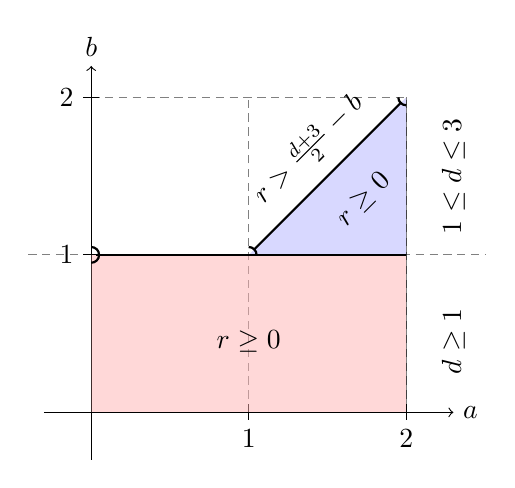
\begin{tikzpicture}[scale=2]
			\draw [->] (-0.3,0) -- (2.3,0) node [right] {$a$};
			\draw [->] (0,-0.3) -- (0,2.2) node [above] {$b$};
			\draw [densely dashed,gray] (1,0) -- (1,2) (2,0) -- (2,2) (-0.4,1) -- (2.5,1) (0,2) -- (2,2);
			\draw (1,0.05) -- (1,-0.05) node [below] {$1$};
			\draw (2,0.05) -- (2,-0.05) node [below] {$2$};
			\draw (0.05,1) -- (-0.05,1) node [left] {$1$};
			\draw (0.05,2) -- (-0.05,2) node [left] {$2$};
			\filldraw [fill=red!30, opacity=0.5] (0,0) rectangle (2,1);
			\filldraw [fill=blue!30, opacity=0.5] (1,1) -- (2,1) -- (2,2);
			\draw [thick] (1.03,1.03) -- (1.97,1.97);
			\draw [thick] ([shift=(0:0.05)]1,1) arc (0:90:0.05);
			\draw [thick] ([shift=(180:0.05)]2,2) arc (180:270:0.05);
			\node at (2.3,1.5) [rotate=90, anchor=center] {$1\le d\le 3$};
			\node at (2.3,0.45)[rotate=90, anchor=center] {$d\ge 1$};
			\draw [thick] (0.03,1) -- (2,1);
			\draw [thick] ([shift=(-90:0.05)]0,1) arc (-90:90:0.05);
			\node at (1.73,1.35) [rotate=45, anchor=center] {$r\ge 0$};
			\node at (1,0.45) {$r\ge 0$};
			% \node at (1,0.9) {$r=0$ or $r>1$};
			\node at (1.5,1.55) [rotate=45,anchor=south] {$r>\frac{d+3}{2}-b$};
			\end{tikzpicture}
		\end{figure}
	\end{frame}
	
	\begin{frame}
		\frametitle{Global Solution\\
			\small $\left(\partial^b_t + \frac{\nu}{2}(-\Delta)^{a/2}\right)\: u(t,x) = I^r_t \left[\sqrt{\theta}\: u(t,x)\: \dot W(x) \right]$}
		\begin{definition}
			$u(t,x)$ is a \textit{global solution} to the {\small (ISHWE)} if $\Norm{u(t,x)}_p < \infty$ for any $t>0$ and $x \in \R^d$.
		\end{definition}
		$\;$ \\
		\begin{theorem}[{\small Chen-E. '21+}]
			A global solution exists provided $G$ is nonnegative and
			\[
			0 < \alpha < \min\left( \frac{a}{b}[2(b+r) -1], 2a, d \right)
			\]
		\end{theorem}
	\end{frame}
	
	\begin{frame}
		\frametitle{Local Solution}
		\begin{definition}
			$u(t,x)$ is a \textit{local solution} to the {\small (ISHWE)} if there exists $0 < T_a \le T_b < \infty$ such that $\Norm{u(t,x)}_2 < \infty$ when $0<t<T_a$ and $\Norm{u(t,x)}_2 $ D.N.E. (does not exist) for $t> T_b$.
		\end{definition}
		$\;$ \\
		\begin{theorem}[{\small Chen-E. '21+}]
			A local solution exists provided $G$ is nonnegative and
			if
			\[
			r\in \left[0,1/2\right] \qquad \text{and} \qquad
			0<\alpha = \frac{a}{b}[2(b+r)-1] \le d.
			\]
			In this case, a unique $L^p(\Omega)$ solution exists for $t \in (0,T_p)$ where
			\[
			T_p := \dfrac{\nu^{\alpha/a}}{2 \theta (p-1) \mathcal{M}_a^{(2a-\alpha)/a}}
			\]
			and the solution does not exist for $t > T_2$.
		\end{theorem}
	\end{frame}
	
	
	
	\begin{frame}[t]
		\frametitle{Example: Solvability for the SWE ($a=b=2$)}
		A local solution only exists when $\alpha = 3+2r \le d \le 3$.
		\begin{figure}[htb]% {{{ F:SWE
			\centering
			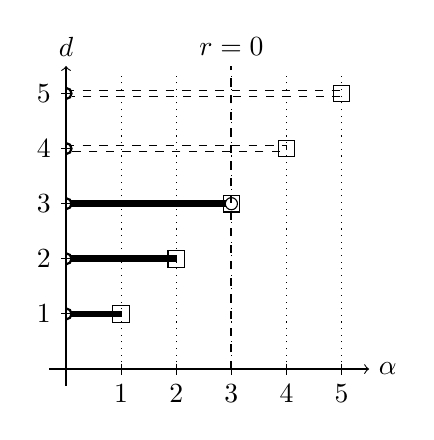
\begin{tikzpicture}[scale=0.7]
			\draw [thick,dashed] (3,0) -- (3,5.5) node [above] {$r=0$};
			\draw [->] (-0.3,0) -- (5.5,0) node [right] {$\alpha$};
			\draw [->] (0,-0.3) -- (0,5.5) node [above] {$d$};
			\foreach \x in {1,...,5}{
				\draw (\x,0.1)--++(0,-0.2) node [below] {$\x$};
				\draw (0.1,\x)--++(-0.2,0) node [left] {$\x$};
				\draw (\x,\x) + (-0.15,-0.15) rectangle +(0.15,0.15);
				\draw [thick] ([shift=(-90:0.1)]0,\x) arc (-90:90:0.1);
				\draw [thin, dotted] (\x,0) -- (\x, 5.4);
			}
			\filldraw (0, 1) + (0.1, -0.05) rectangle +(1,0.05);%\filldraw (1,1) circle (0.05);
			\filldraw (0, 2) + (0.1, -0.05) rectangle +(2,0.05);%\filldraw (2,2) circle (0.05);
			\filldraw (0, 3) + (0.1, -0.05) rectangle +(2.9,0.05);%\filldraw (3,3) circle (0.05);
			% \filldraw (0, 4) + (0.1, -0.05) rectangle +(2.9,0.05);
			% \filldraw (0, 5) + (0.1, -0.05) rectangle +(2.9,0.05);
			% \draw (2,2) circle (0.11);
			\draw (3,3) circle (0.11);
			% \draw (3,4) circle (0.11);
			% \draw (3,5) circle (0.11);
			% \draw (2, 3) + (0.1, -0.05) rectangle +(1,0.05);
			% \draw (2, 4) + (0.1, -0.05) rectangle +(2,0.05);
			\draw[dashed] (0, 5) + (0.1, -0.05) rectangle +(5,0.05);
			\draw[dashed] (0, 4) + (0.1, -0.05) rectangle +(4,0.05);
			\end{tikzpicture}
			\hspace{2em}
			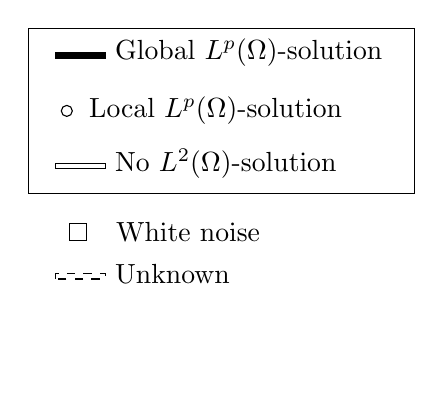
\begin{tikzpicture}[scale=0.7]
			\def\x{3.2}
			% \draw (-0.4,-1.5+\x) rectangle +(6,3);
			% \draw (0.5,0+\x) circle (0.1); \node at (3,0+\x) {Local $L^p(\Omega)$-solution};
			% \draw (0, -1+\x) + (0.1, -0.05) rectangle +(1,0.05) node [right] {No $L^2(\Omega)$-solution};
			% \draw (0.5, 1) + (-0.15,-0.15) rectangle +(0.15,0.15); \node at (2.5,1) {White noise};
			\draw[dashed] (0, -3+\x) + (0.1, -0.05) rectangle +(1,0.05) node [right] {Unknown};
			\draw (-0.4,-1.5+\x) rectangle +(7,3);
			\filldraw (0, 1+\x) + (0.1, -0.05) rectangle +(1,0.05) node [right] {Global $L^p(\Omega)$-solution};
			\draw (0.3,0+\x) circle (0.1); \node at (3,0+\x) {Local $L^p(\Omega)$-solution};
			\draw (0, -1+\x) + (0.1, -0.05) rectangle +(1,0.05) node [right] {No $L^2(\Omega)$-solution};
			\draw (0.5, 1) + (-0.15,-0.15) rectangle +(0.15,0.15); \node at (2.5,1) {White noise};
			\draw[white] (0,-1.5) circle (0.01);
			\end{tikzpicture}
		\end{figure}% }}}
		By replacing $\nu=2$ in the following, we recover (1.12) {\small [Balan, L. Chen \& X. Chen '21]}
		\[
		T_p=	\frac{\nu^{3 / 2}}{2\theta (p-1) \sqrt{\mathcal{M}_{2,3}(\delta_0)}},  \quad p\ge 2
		\]
	\end{frame}
	
	
	\begin{frame}[t]
		\frametitle{Example: Solvability for the SHE ($a=2$ and  $b=1$)}
		By setting $a=2$, $b=1$ and $r=0$, we obtain the following condition for existence of a local solution: $\alpha = 2 \le d.$
		\begin{columns}
			\begin{column}{0.5\textwidth}
				\begin{figure}[htpb]% {{{ F:SHE
					\centering
					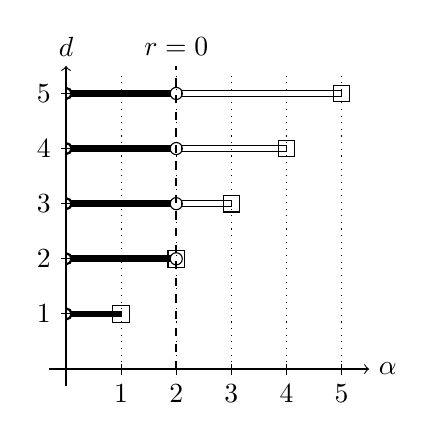
\begin{tikzpicture}[scale=0.7]
					\draw [thick,dashed] (2,0) -- (2,5.5) node [above] {$r=0$};
					\draw [->] (-0.3,0) -- (5.5,0) node [right] {$\alpha$};
					\draw [->] (0,-0.3) -- (0,5.5) node [above] {$d$};
					\foreach \x in {1,...,5}{
						\draw (\x,0.1)--++(0,-0.2) node [below] {$\x$};
						\draw (0.1,\x)--++(-0.2,0) node [left] {$\x$};
						\draw (\x,\x) + (-0.15,-0.15) rectangle +(0.15,0.15);
						\draw [thick] ([shift=(-90:0.1)]0,\x) arc (-90:90:0.1);
						\draw [thin, dotted] (\x,0) -- (\x, 5.4);
					}
					\filldraw (0, 1) + (0.1, -0.05) rectangle +(1,0.05);%\filldraw (1,1) circle (0.05);
					\filldraw (0, 2) + (0.1, -0.05) rectangle +(1.9,0.05);
					\filldraw (0, 3) + (0.1, -0.05) rectangle +(1.9,0.05);
					\filldraw (0, 4) + (0.1, -0.05) rectangle +(1.9,0.05);
					\filldraw (0, 5) + (0.1, -0.05) rectangle +(1.9,0.05);
					\draw (2,2) circle (0.11);
					\draw (2,3) circle (0.11);
					\draw (2,4) circle (0.11);
					\draw (2,5) circle (0.11);
					\draw (2, 3) + (0.1, -0.05) rectangle +(1,0.05);
					\draw (2, 4) + (0.1, -0.05) rectangle +(2,0.05);
					\draw (2, 5) + (0.1, -0.05) rectangle +(3,0.05);
					\end{tikzpicture}
				\end{figure}
			\end{column}
			\begin{column}{0.5\textwidth}
				\begin{itemize}
					\item 	When $\alpha=d=2$, the critical time becomes $T_p = \dfrac{\nu}{2\theta (p-1) \mathcal{M}_{2,2}(\delta_0)}$.
					\item Theorem 4.1 {\small [Y. Hu, '01]} proves that an $L^2(\Omega)$ solution exists for $t<2$ but not for $t>2 \pi$.
					\item $T_2$ being precise implies $2 \le T_2 = \frac{1}{2\mathcal{M}_{2,2}(\delta_0)} \le 2\pi$
				\end{itemize}
			\end{column}
		\end{columns}
		
	\end{frame}
	
	\begin{frame}[t]
		\frametitle{Wiener Chaos Expansion}
		
		Through a standard procedure, we may define
		\[
		f_n(x_1, \cdots , x_n; x, t) = \int_0^t\int_0^{t_n}\cdots \int_0^{t_2} \prod_{k=1}^n G(t_{k+1}-t_k,x_{k+1}-x_k) \ud t_1 \cdots \ud t_n
		\]
		where $t=t_{n+1}$ and $x=x_{n+1}$, and say that
		\vspace{1em}
		\begin{enumerate}
			\setlength\itemsep{.8em}
			\item $u(t,x) = 1 + \sum_{k=1}^\infty \theta^{k/2} I_k(f_k(\cdot,x,t)), \quad (t,x)\in (0,T)\times \R^d$
			
			\item $\mathbb{E}(u(t,x)^2) = \sum_{k=0}^\infty \theta^{k} \Norm{f_k(\cdot,x,t)}^2_{\mathcal{H}^{\otimes n}}, \quad (t,x)\in (0,T)\times \R^d$.
		\end{enumerate}
		\vspace{1em}
		Through a change of variable, one can easily show that
		\vspace{1em}
		\begin{enumerate}
			\item $\mathcal{F}G(t,\cdot)(c\xi) = c^{-\frac{a}{b}(b+r -1)}\mathcal{F}G\left(c^{\frac{a}{b}}t,\cdot\right)( \xi)$
			\item $\Norm{\widetilde{f_n}(\cdot,0,t)}_{\mathcal{H}^{\otimes n}}^2 = t^{[2(b + r ) -b \alpha / a]n} \Norm{\widetilde{f_n}(\cdot,0,1)}_{\mathcal{H}^{\otimes n}}^2$
		\end{enumerate}
	\end{frame}
	
	\begin{frame}[t]
		\frametitle{How to Find the Critical $\alpha$}
		For simplicity we consider the SWE ($a=b=2$ and $r=0$).
		\begin{align*}
		\Norm{u(t,x)}_2^2 &= \sum_{n \ge 0} \theta^n n! \: \overbrace{t^{[4 - \alpha ]n}  \Norm{ \widetilde{f_n}(\cdot,0,1) }_{ \mathcal{H}^{\otimes n} }^2}^{\Norm{ \widetilde{f_n}(\cdot,0,t) }_{ \mathcal{H}^{\otimes n} }^2}
		\\&= \sum_{n \ge 0} \frac{\theta^nt^{(4-\alpha)n}}{(n!)^{3-\alpha}} R_n, \quad R_n = (n!)^{4-\alpha}\Norm{\widetilde{f}_n(\cdot,0,1)}_{\mathcal{H}^{\otimes n}}^2
		\end{align*}
		When $\alpha = 3$, then the above reduces down to
		\[
		\Norm{u(t,x)}_2^2 =  \sum_{n \ge 0} (\theta t)^n n! \Norm{ \widetilde{f_n}(\cdot,0,1) }_{ \mathcal{H}^{\otimes n} }^2.
		\]
		and we lose the $n!$ term in the demonstrator.
	\end{frame}
	
	\begin{frame}[t]
		\frametitle{$\rho$}
		We define
		\begin{align*}
		\rho_{\nu,a}(\gamma) &= \sup_{\Norm{f}_{L^2(\R^d)} =1} \int_{\R^d} \left[ \int_{\R^d} \frac{f(x+y)f(y)}{\sqrt{1+\frac{\nu}{2}|x+y|^a } \sqrt{1+\frac{\nu}{2}|y|^a} } \ud y \right]^2 \mu(\ud x)
		\end{align*}
		
		
		
		
		\begin{theorem}[{\small X. Chen '07}]
			\begin{align*}
			\lim_{n \to \infty} \frac{1}{n} \log & \left[ \frac{1}{(n!)^2} \int_{(\R^d)^n} \left( \sum_{\sigma \in \Sigma_n} \prod_{k=1}^n \frac{1}{1+ \frac{\nu}{2}|\sum_{j=k}^n \xi_{\sigma(j)}|^a}\right)^2 \mu (\ud \vec{\xi})\right]
			\\& = \log\left( \rho_{\nu, a}\left(\gamma\right) \right).
			\end{align*}
			where $\gamma$ is the spatial correlation function.
		\end{theorem}
		
	\end{frame}
	
	\begin{frame}[t]
		\frametitle{Connection of the SPDE with $\rho$}
		Recall from above that
		\[
		\mathcal{F}\mathcal{L}G(1,\xi) = \frac{1}{1+\frac{\nu}{2}|\xi|^a}.
		\]
		By using this relation, it can be shown that
		\[
		\mathcal{F}\mathcal{L}(\tilde{f}_n)(1,\xi) = \frac{1}{n!} \sum_{\sigma \in \Sigma_n} \prod_{k=1}^n \frac{1}{1+ \frac{\nu}{2}|\sum_{j=k}^n \xi_{\sigma(j)}|^a}.
		\]
		Applying this to the limit representation of $\rho$ above yields that
		\begin{align*}
		\lim_{n \to \infty} \frac{1}{n} \log  \left[ \int_{(\R^d)^n} \left| \mathcal{F}\mathcal{L}(\tilde{f}_n)(1,\xi)\right|^2 \mu (\ud \vec{\xi})\right]  = \log\left( \rho_{\nu, a}\left(\gamma\right) \right).
		\end{align*}
	\end{frame}
	
	\begin{frame}
		
		
		Recall the scaling property
		\[
		\Norm{\tilde{f}_n(\cdot,0,t)}_{\mathcal{H}^{\otimes n}}^2 = t^{(4-\alpha)n}\Norm{\tilde{f}_n(\cdot,0,1)}_{\mathcal{H}^{\otimes n}}^2.
		\]
		Using this scaling property we see that
		\[
		\int_0^\infty e^{-t}\Norm{\tilde{f}_n(\cdot,0,t)}_{\mathcal{H}^{\otimes n}}^2  \ud t = \Gamma((4-\alpha)n+1)\Norm{\tilde{f}_n(\cdot,0,1)}_{\mathcal{H}^{\otimes n}}^2.
		\]
		
		\begin{lemma}[{\small R.  Balan, L. Chen \& X. Chen '21}]
			
			\begin{align*}
			\lim_{n \to \infty}\frac{1}{n} \log & \left(\Gamma((4-\alpha)n+1)\Norm{\tilde{f}_n(\cdot,0;1)}_{\mathcal{H}^{\otimes n}}^2\right) = \log\left[ 2^{4-\alpha}\rho \right]
			\\ \\ \lim_{n \to \infty}\frac{1}{n} \log & \left((n!)^{4-\alpha}\Norm{\tilde{f}_n(\cdot,0;1)}_{\mathcal{H}^{\otimes n}}^2\right) = \log\left[ \left(\frac{2}{4-\alpha}\right)^{4-\alpha}\rho \right]
			\end{align*}
		\end{lemma}
	\end{frame}
	
	\begin{frame}[t]
		\frametitle{How to Find the Blowup Time (SWE)}
		Recall from above that the critical case corresonds to $\alpha = 3 = d$.
		\begin{align*}
		\Norm{u(t,x)}_2^2 &= \sum_{n \ge 0} \theta^n n! \Norm{\tilde{f}(\cdot,0,t)}_{H^{\otimes n}}^2
		\\&= \sum_{n \ge 0} (\theta t)^n n! \Norm{\tilde{f}(\cdot,0,1)}_{H^{\otimes n}}^2
		\\& =: \sum_{n \ge 0} (\theta t)^n R_n, \quad R_n = n! \Norm{\tilde{f}(\cdot,0,1)}_{H^{\otimes n}}^2.
		\end{align*}
		The above lemma says that $\frac{1}{n}\log{R_n} \to \log(2 \rho_c)$. Now the Cauchy-Hadamard theorem can be directly applied to see that the radius of convergence is precisely $(2\theta \rho_c)^{-1} = T_2$.
		
	\end{frame}
	
	\begin{frame}[t]% {{{ M
		\frametitle{$\mathcal{M}$}
		We define
		\begin{align*}
		\mathcal{M}_{a,d}(\gamma,\theta) & := \sup_{g \in \mathcal{F}_a} \left\{ \left( \iint_{\R^{2d}} g^2(x)g^2(y) \gamma(x+y)\ud x\ud y \right)^{1/2} - \frac{\theta}{2}\: \mathcal{E}_a(g,g) \right\} \\
		& = \sup_{g \in \mathcal{F}_a} \left\{ \left\langle g^2 * g^2, \gamma \right\rangle_{L^2(\R^d)}^{1/2} - \frac{\theta}{2}\: \mathcal{E}_a(g,g) \right\},
		\end{align*}
		where
		\begin{gather*}
		\mathcal{E}_a(g,g) := (2\pi)^{-d} \int_{\R^d} |\xi|^a |\mathcal{F}g(\xi)|^2 \ud \xi \quad \text{and} \\
		\mathcal{F}_a      := \left\{f\in L^2(\R^d): \: \Norm{f}_{L^2(\R^d)}=1,\: \mathcal{E}_a(f,f)<\infty \right\}.
		\end{gather*}
	\end{frame}% }}}
	
	\begin{frame}% {{{ Connection between rho and M
		\frametitle{The Connection between $\rho$ and $\mathcal{M}$}
		Recall that
		\begin{align*}
		\rho_{\nu,a}(\gamma) &= \sup_{\Norm{f}_{L^2(\R^d)} =1} \int_{\R^d} \left[ \int_{\R^d} \frac{f(x+y)f(y)}{\sqrt{1+\frac{\nu}{2}|x+y|^a } \sqrt{1+\frac{\nu}{2}|y|^a} } \ud y \right]^2 \mu(\ud x).
		\end{align*}
		
		\begin{theorem}[{\small Bass, X. Chen and Rosen '09}]
			\[
			\rho_{\nu,a}(\gamma) = \nu^{-\alpha/a} \mathcal{M}_a^{2-(\alpha / a)}(\gamma)<\infty
			\]
		\end{theorem}
	\end{frame}% }}}
	
	\begin{frame}[t]% {{{ Moment asymptotics
		\frametitle{The Moment Asymptotic}
		\begin{theorem}[{\small Chen-E. '21+}]
			Suppose a global solution to the SPDE in question exists and $\dot{W}$ is given through the generalized Riesz kernel defined above. Then,
			\begin{align*}
			\lim_{t_p \to \infty} & t_p^{-\beta} \log \Norm{u(t,x)}_p                                          \\
			& =  \left(\frac{1}{2}\right)\left(\frac{2a}{2a(b+r)- b\alpha} \right)^\beta \\
			& \quad \quad \quad  \times \left(\theta\nu^{-\alpha/a} \mathcal{M}_a^{\frac{2a-\alpha}{a}}\right)^{\frac{a}{2a(b+r)-b\alpha-a}}\left(2(b+r)-\frac{b\alpha}{a}-1\right),
			\end{align*}
			where
			\begin{align*}
			% \label{E:beta-tp}
			\beta := \dfrac{2(b+r)-\dfrac{b\alpha}{a}}{ 2(b+r)-\dfrac{b\alpha}{a} -1 } \qquad \text{and} \qquad
			t_p   := (p-1)^{1-1/\beta} \: t.
			\end{align*}
		\end{theorem}
	\end{frame}% }}}
	
	\begin{frame}[t]% {{{ Exponential growth of moments in time
		% \frametitle{Exponential Growth of the Moments in Time}
		\frametitle{Exact Moment Lyapunov Exponent \\
			\small (Recall $\beta := \frac{2(b+r)-\frac{b\alpha}{a}}{ 2(b+r)-\frac{b\alpha}{a} -1}$)}
		\begin{corollary}[{\small Chen-E. '21+}]
			For $p \ge 2$ fixed, we have that
			\begin{align*}
			\lim_{t \to \infty} & t^{-\beta} \log \E\left(|u(t,x)|^p\right)                                                                                 \\
			& =  p(p-1)^{\frac{1}{2(b+r)-\frac{b\alpha}{a} -1}} \left(\frac{1}{2}\right)\left(\frac{2a}{2a(b+r)- b\alpha} \right)^\beta \\
			& \quad \quad \times \left(\theta\nu^{-\alpha/a} \mathcal{M}_a^{\frac{2a-\alpha}{a}}\right)^{\frac{a}{2a(b+r)-b\alpha-a}}\left(2(b+r)-\frac{b\alpha}{a}-1\right).
			\end{align*}
		\end{corollary}
		\vfill
		
		From this we can deduce that $t \mapsto \mathbb{E}(|u(t,x)|^p)$ will grow like $\exp\left({K_1 t^\beta }\right)$, in other words, the moments will grow exponentially in time,
		and we obtain the exact expression for the constant $K_1$.
	\end{frame}% }}}
	
	\begin{frame}[t]% {{{ Exact Large Moment Asymptotics
		% \frametitle{Exponential Growth of the moments for Fixed Time}
		\frametitle{Exact Large Moment Asymptotics \\
			\small (Recall $\beta := \frac{2(b+r)-\frac{b\alpha}{a}}{ 2(b+r)-\frac{b\alpha}{a} -1}$)}
		\begin{corollary}[{\small Chen-E. '21+}] For $t>0$ fixed , we have that
			\begin{align*}
			\lim_{p \to \infty} & p^{-\beta} \log \E\left(|u(t,x)|^p\right)                                          \\
			& =  t^\beta \left(\frac{1}{2}\right)\left(\frac{2a}{2a(b+r)- b\alpha} \right)^\beta \\
			& \quad \quad \times \left(\theta\nu^{-\alpha/a} \mathcal{M}_a^{\frac{2a-\alpha}{a}}\right)^{\frac{a}{2a(b+r)-b\alpha-a}}\left(2(b+r)-\frac{b\alpha}{a}-1\right).
			\end{align*}
		\end{corollary}
		\vfill
		
		From this we can deduce that $p \mapsto \mathbb{E}(|u(t,x)|^p)$ will grow like $\exp\left({K_2 p^\beta }\right)$, in other words, the moments will grow exponentially in $p$ as well.
		
	\end{frame}% }}}
	
	\begin{frame}
		\frametitle{End}
		\begin{center}
			Thank you for listening!
		\end{center}
	\end{frame}
	
	\begin{frame}
		\frametitle{References}
		\small
		
		\begin{thebibliography}{999}
			\bibitem{BCC21} % {{{ 1.
			Balan, R. M., Chen, L., and Chen, X. (2021).
			\newblock Exact asymptotics of the stochastic wave equation with time-independent noise.
			\newblock {\em  Ann. Inst. Henri Poincar\'e Probab. Stat. }, to appear.
			
			\bibitem{BCR09}% {{{ 2.
			Bass, R., Chen, X., and Rosen, M. (2009).
			\newblock Large deviations for Riesz potentials of additive processes.
			\newblock {\em  Ann. Inst. Henri Poincar\'e Probab. Stat. } \textbf{45}, 626--666.
			% }}}
			
			\bibitem{BCC21} % {{{ 1.
			Chen, L. and Eisenberg, N. (2021+).
			\newblock Interpolating the Stochastic Heat and Wave Equations\\ with Time-independent Noise:Solvability and Exact Asymptotics
			\newblock {\em  arXiv:2108.11473}, submitted.
			
			\bibitem{Chen17AIHP} % {{{ 6.
			Chen, X. (2017).
			\newblock Moment asymptotics for parabolic Anderson equation with fractional time-space noise: in Skorohod regime.
			\newblock {\em Ann. Inst. Henri Poincar\'e: Prob. Stat.} {\bf 53} 819--841.
			
		\end{thebibliography}
	\end{frame}
	
	\begin{frame}[t]
		\frametitle{References}
		\small
		
		\begin{thebibliography}{999}
			\bibitem{Hu01Heat} % {{{ 6.
			Hu, Y. (2001).
			\newblock Heat equation with fractional white noise potential.
			\newblock {\em Appl. Math. Optim.} {\bf 20} 221--243.
			% }}}
		\end{thebibliography}
	\end{frame}
	
	\begin{frame}[t]
		\frametitle{Anticipated Question: Finiteness of $\rho$}
		Recall $\varphi(x) = \prod_{i=1}^n|x_{(i)}|^{d_i-\alpha_i}$. By examining Lemma 1.6 (X. Chen 2007), to show $\rho$ is finite for the generalized Riesz kernel, then we need to prove the following:
		\[\int_{\R^d}\int_{\R^d} F(y)G(x)\varphi(x-y) \ud y \ud x \le C \Norm{F}_{2d/(d+\alpha)} \Norm{G}_{2d/(d+ \alpha)}\]
		This can be done by using weak Young's inequality
		\[
		\left|	\int_{\R^d}\int_{\R^d}a(x)b(x-y)c(y) \ud x \ud y \right| \le K_{p,q,r,d} \Norm{a}_p\Norm{b}_{q,w}\Norm{c}_r
		\]
		where $q^{-1} + q'^{-1} = 1$ and $p^{-1}+q^{-1}+r^{-1} =2$ and
		\[
		\Norm{b}_{q,w} = \sup_{A} |A|^{-1/q'} \int_A |b(x)| \ud x, \quad |A| < \infty.
		\]
		We apply this with
		\[
		a=F, \quad b=\varphi, \quad c= G
		\]
		and we show that $\Norm{\varphi}_{q,w} < \infty$ with $q=d/(d-\alpha)$.
	\end{frame}
	
	
	\begin{frame}
		\frametitle{Anticipated Question: Why does $\rho$ appear in the Lemma.}
		
		For simplicity we will consider the second moments of stochastic wave equation ($a=b=2$ and $r=0$). We will also only consider the limit
		\[
		\lim_{n \to \infty}\frac{1}{n} \log\left(\Gamma((4-\alpha)n+1)\Norm{\tilde{f}_n(\cdot,0;1)}_{\mathcal{H}^{\otimes n}}^2\right) = \log\left[ 2^{4-\alpha}\rho \right]
		\]
		Recall that
		\[
		\int_0^\infty e^{-t}\Norm{\tilde{f}_n(\cdot,0,t)}_{\mathcal{H}^{\otimes n}}^2  \ud t = \Gamma((4-\alpha)n+1)\Norm{\tilde{f}_n(\cdot,0,1)}_{\mathcal{H}^{\otimes n}}^2.
		\]
		Define $T_n:= \int_{(\R^d)^n} \left| \mathcal{F}\mathcal{L}\tilde{f}_n(1,\xi)\right|^2 \mu (\ud \vec{\xi})$. Through direct calculation and Sterlings formula:
		\begin{align*}
		\frac{c_\alpha}{C_n} 2^{(4-\alpha)n}T_n \le \int_0^\infty e^{-t} \Norm{\tilde{f}(\cdot,0,t)}_{H^{\otimes n}}^2 \ud t  \le 2^{(4-\alpha)n}T_n
		\end{align*}
		Where $\log(C_n)/n \to 0$ and $c_\alpha >0$.
	\end{frame}
	
	\begin{frame}[t]
		\frametitle{Anticipated Question: Finding the moment asymptotic}
		\begin{align*}
		\mathbb{E}(|u(t,x)|^2) = \sum_{n \ge 0} z_n R_nt^{(2(b+r)-b\alpha/a)n}
		\end{align*}
		\begin{align*}
		R_n = (n!)^{2(b+r)-b\alpha/a}\Norm{\widetilde{f}_n(\cdot,0,1)}_{\mathcal{H}^{\otimes n}}^2 \quad \text{and} \quad
		z_n = \frac{\theta^n}{(n!)^{2(b+r)-(b\alpha/a)-1}}.
		\end{align*}
		\begin{align*}
		\frac{1}{n}\log(R_n) \to  \log\left( \left(\frac{2}{2(b+r)-\frac{b\alpha}{a}}\right)^{2(b+r)-\frac{b\alpha}{a}}  \rho \right )  \quad \text{as } n\to \infty.
		\end{align*}
		If we find a $\beta$ and $A$ so that
		\begin{align*}
		\lim_{t \to \infty}\frac{1}{t^\beta} \log \sum_{n \ge 0} z_n R^n \left(t^{(2(b+r)-b\alpha/a)}\right)^n = A.
		\end{align*}
		then this is implies
		\begin{align*}
		\lim_{t \to \infty}\frac{1}{t^\beta} \log \sum_{n \ge 0} z_n R_n \left(t^{(2(b+r)-b\alpha/a)}\right)^n = A.
		\end{align*}
	\end{frame}
\end{document}
